\documentclass[a4paper, titlepage]{article}

\usepackage[utf8]{inputenc}
\usepackage{courier} % Required for the courier font
\usepackage[bookmarks]{hyperref}
\usepackage{graphicx}
\usepackage{filecontents}

%redefine percentage sign to be a little smaller
\let\oldpct\%
\renewcommand{\%}{\scalebox{.9}{\oldpct}}

\setcounter{secnumdepth}{0}
\begin{document}

\title{Probabilistic modelling of text-input, facilitating uncalibrated
gaze-typing}
\author{
	Sigurt Bladt Dinesen
	\\\texttt{sidi@itu.dk}
	\and
	Advisor:
	\\Dan Witzner Hansen
}


\maketitle
\tableofcontents

\clearpage

\section{Abstract}

\section{Introduction}
The purpose of this project is to explore the use of language- and
input-models, meant to facilitate eye typing with uncalibrated eye tracking.

Typing is a ubiquitous input method for human-computer interaction, particularly for human-to-human communication facilitated by computers.

Several methods have been developed to help humans type faster and more
accurately, especially on mobile platforms like mobile phones. Some
methods are based on probabilistic language- and input-modelling, such
as T9 and the replace-as-you-type technologies (colloquially;
\emph{autocorrect}) that have mostly replaced T9 on contemporary
smartphones, perhaps due to widespread deployment of touchscreens. Other
methods use gestures, or leverage creative arrangements of input
symbols. Examples include swype for Android and IOS, and Dasher and
StarGazer intended for use with eye tracking.

The use of eye tracking as a means of text input (eye typing) can be
demanding on the user. Exact and deliberate control of the gaze is
difficult and tiring, and in addition to the energy expended when
typing, most systems require users to go through calibration routines
before use.

One area where eye typing has seen use is as a communication platform
for ALS (amyotrophic lateral sclerosis) patients. Patients suffering
suffering from ALS often retain the use of their eye muscles longer than
that of other muscles, and eye typing can therefore help increase their
quality of life. In practice, patients tend to use eye typing
for short commands and answers. For such usage patterns, uncalibrated
eye typing will be particularly beneficial.

To explore facilitation of uncalibrated tracking, the following work is
presented:
\begin{enumerate}
\item
  A language- and input-model is presented, in order
  to make educated guesses as to the intended user input, in an attempt
  to compensate for tracker (and user) imprecisions. In particular, the goal of
  the models is to ease typing by accepting mistakes, to lessen the need of
  typing, by guessing future inputs.
\item
  A typing system is implemented, as a simulation using a
  pointing device (mouse). To solve the problem known as
  \emph{midas touch}, input symbols continuously move along the perimeter of a
  circle. This movement is then correlated with the user input.
\item
  The typing system is evaluated in an informal typing-speed experiment.
\end{enumerate}

The deliverables of is project are software implementations of the
language- and input-model, of the eye typing system(s), and a report
detailing the project process and results.

\section{Background}
The efficacy of using moving targets to avoid the problem of unintended
activations (Midas touch) in Gaze-input systems has been established for
controls in Pursuits\cite{pursuits} and Orbits\cite{orbits}, and for general
text-input in Dasher \cite{dasher} and StarGazer\cite{stargazer}. The former two
using the correlation between user eye-movement and controls for selection,
while the latter two "zoom in" on targets, gradually excluding selections that
appear uninteresting to the user.

Moving targets on circular trajectories allows selection between multiple
targets, without requiring a calibration phase\cite{pursuits,orbits}, by
calculating the Pearson's product-moment correlation between the corresponding
x- and y-coordinates of the users gaze points, and the positions of each target.

\section{Apparatus}
The setup simulates a gaze tracking system, accepting the mouse-cursor
coordinates as inputs, as if they where from an gaze tracker. The cursor is
controlled using the built-in touchpad on a 2014-model lenovo x1.
The choice to simulate a gaze tracker with a touchpad is significant. As a
result, the typing speed of this system cannot be compared to that of systems
that use gaze trackers. The typing speed with and without predictive language
modelling can still be compared internally to this project however.

The text typed by the user is simply displayed in a console (shown at the
bottom in figure \ref{fig:apparatus}, with a "$\vert$" indicating the position
of the next letter (the intention is to let the user see if the texts ends with
a space of not). While this method of visualizing the text is not particularly
elegant, it is sufficient for our purposes.

User inputs are sampled at the frame rate used to display the interface, 60 hz.
The high input rate may artificially increase the systems accuracy, but since
direct comparison to systems based on gaze tracking is not the goal, little
attention has been given to the precise hardware parameters.

\begin{figure}[htbp]
  \centering
    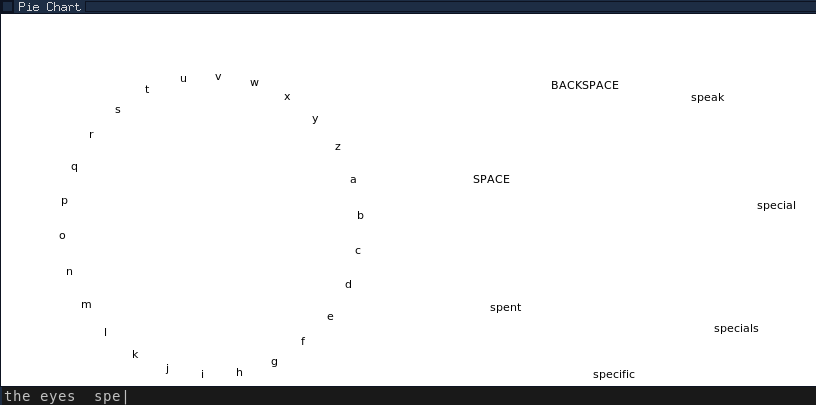
\includegraphics[width=0.95\textwidth]{screenshot.png}
  \caption{}
  \label{fig:apparatus}
\end{figure}

\section{Project Design}
The system consists of two parts; an input that interprets the sequence of x-
and y-coordinates the user inputs, and a language model that tries to guess what the user wants to type next, based on previous inputs.

\section{Input model}
Closely inspired by Orbits\cite{orbits}, the targets are displayed moving along
the periphery on two circles (refer back to figure \ref{fig:apparatus} for an
illustration). The targets on the left circle follow a clockwise trajectory,
while the targets on the right circle follow a counterclockwise trajectory.

The left circle contains the letters of the English alphabet, while the right
circle holds meta-characters \texttt{SPACE} and \texttt{BACKSPACE} -- used to
insert a white-space or delete a character respectively -- and any predictions
made by the language model.

Like Pursuits and Orbits \cite{pursuits,orbits}, I use Pearson's
product-moment correlation between target and user-gaze trajectories to
determine which target the user is trying to select, if any.

In order to determine the correlation, it is necessary to maintain a
time-window of trajectories. 

Defining a trajectory $t_{1 \dots n}$ such that $t_i$ is the coordinate for $t$
at the $i$'th position in a timewindow of size $n$, the Pearson's product-moment
correlation between two trajctories $x$ and $y$ can be defined as:
$$\frac{\sum\limits_{i=1}^n (x_i - \bar x)(y_i - \bar y)}
{\sqrt{\sum\limits_{i=1}^n (x_i - \bar x)^2} \sqrt{\sum\limits_{i=1}^n (y_i - \bar y)^2}}$$

In English, this gives us covariance of two trajectories, divided by the product
of their standard deviations. Intuitively function value grows when $x$ and $y$
deviate in the same direction from their means, at the same point in time.

At every frame, each target in the two circles has its trajectory correlated
with the usergaze trajectory, using the formula. This is done twice for each
target, once for for x-coordinates and once for y-coordinates. The correlation
for the target is taken to be the minimum of its x and y correlations. This way,
for a target to have a high correlation with the user gaze trajectory, the
trajectories must have a high correlation on both the horizontal and vertical
axes.

 Esteves et al.\cite{orbits} found that a window size of 30 samples,
corresponding to 1 second's worth of inputs, works well. I used a window size of
90 samples, corresponding to 1.5 second at 60 samples per second. The targets
move at 60 degrees/sec, compared to 120 degrees/sec in Orbits. I found that the
slower speed accommodates the use of a touchpad well.

Similarly, the number of targets displayed would be far to high for a use with a
gaze tracker, based on the findings of Esteves et al.\cite{orbits}, who found
that the rate of true positives dropped significantly when they went from 8 to 16
targets.

\section{Language model}
While I would have liked to explore language models that help allow erroneous
selections in the input model, only one language model has been implemented.
While it doesn't help fix mistakes, it can help prevent them, by requiring fewer
selections to be made by the user.

The model combines two Markov models of order 0 and 3 respectively
using a large body of email texts as training set.

The models use full words as the definition of "state". That is; the 3'rd order
Markov model ("context model" hereafter) predicts the next word, based on a 3 word context, whereas the
0'th order Markov model ("word model" hereafter) predicts the next word based on no context.

The intuition behind using two models is that while the context model
can make predictions based on sentence context, it can often falls short.
The word model is useful when;
\begin{itemize}
	\item less than 3 words of context exist, or
	\item the 3 word context passes a sentence boundary (the model is
		trained without regard for such boundaries), or
	\item few or no predictions are made by the context, or
	\item the user has typed the first few letters of a word, and they are
		not a prefix of any of the predictions made by the context model.
\end{itemize}

Note that the word model is essentially just a list of words known
to the model, ordered by the frequency with which they occur in the training
set.

Concretely, the predictive model works by taking a three word context.
If the user is in the middle of typing a word, the unfinished word is passed to
the model in addition to the 3 word context.
The model then takes all words that the context model suggests with
non-zero probability, removing those that the unfinished word is not a prefix of
(the case where there is no unfinished word is modelled naturally by letting the
empty string be a prefix of all strings). It then does the same for the word
model. The suggestion lists from the two models are individually sorted by their
respective model's confidence in the results. Only the 5 best predictions are
chosen, taken first from the context Model's suggestions. This ensures that the
word model is doesn't dominate the predictions as it otherwise would, given that
the frequency of a word occurring at all in the training set will generally be
higher than the frequency of that same word occurring in a given context.

\subsection{Training Data}

\section{User study}
wpm vs: san augustin (p4453), dasher (p19-t), p2421, san augustin (p77)
no model: "my watch fell in the water prevailing" 5 min 30 sec, 11 errors.
7 words 38 chars
model: "my watch fell in the water prevailing wind from the east never to" 5min
30 sec, 7 errors. 13 words, 66 chars.

\section{Conclusion}

%\newpage

\begin{filecontents}{mybib.bib}
@inproceedings{dasher,
 author = {Tuisku, Outi and Majaranta, P\"{a}ivi and Isokoski, Poika and R\"{a}ih\"{a}, Kari-Jouko},
 title = {Now Dasher! Dash Away!: Longitudinal Study of Fast Text Entry by Eye Gaze},
 booktitle = {Proceedings of the 2008 Symposium on Eye Tracking Research \&\#38; Applications},
 series = {ETRA '08},
 year = {2008},
 isbn = {978-1-59593-982-1},
 location = {Savannah, Georgia},
 pages = {19--26},
 numpages = {8},
 url = {http://doi.acm.org/10.1145/1344471.1344476},
 doi = {10.1145/1344471.1344476},
 acmid = {1344476},
 publisher = {ACM},
 address = {New York, NY, USA},
 keywords = {eye tracking, gaze writing, longitudinal study, text entry},
} 

@inproceedings{orbits,
 author = {Esteves, Augusto and Velloso, Eduardo and Bulling, Andreas and Gellersen, Hans},
 title = {Orbits: Gaze Interaction for Smart Watches Using Smooth Pursuit Eye Movements},
 booktitle = {Proceedings of the 28th Annual ACM Symposium on User Interface Software \&\#38; Technology},
 series = {UIST '15},
 year = {2015},
 isbn = {978-1-4503-3779-3},
 location = {Charlotte, NC, USA},
 pages = {457--466},
 numpages = {10},
 url = {http://doi.acm.org/10.1145/2807442.2807499},
 doi = {10.1145/2807442.2807499},
 acmid = {2807499},
 publisher = {ACM},
 address = {New York, NY, USA},
 keywords = {eye tracking, gaze input, gaze interaction, pursuits, small devices, small displays, smart watches, wearable computing.},
}

@inproceedings{pursuits,
 author = {Vidal, M{\'e}lodie and Bulling, Andreas and Gellersen, Hans},
 title = {Pursuits: Spontaneous Interaction with Displays Based on Smooth Pursuit Eye Movement and Moving Targets},
 booktitle = {Proceedings of the 2013 ACM International Joint Conference on Pervasive and Ubiquitous Computing},
 series = {UbiComp '13},
 year = {2013},
 isbn = {978-1-4503-1770-2},
 location = {Zurich, Switzerland},
 pages = {439--448},
 numpages = {10},
 url = {http://doi.acm.org/10.1145/2493432.2493477},
 doi = {10.1145/2493432.2493477},
 acmid = {2493477},
 publisher = {ACM},
 address = {New York, NY, USA},
 keywords = {correlation, eye movement, eye-based interfaces, smooth pursuits, spontaneous interaction},
}

@inproceedings{wlowcost,
 author = {San Agustin, Javier and Skovsgaard, Henrik and Hansen, John Paulin and Hansen, Dan Witzner},
 title = {Low-cost Gaze Interaction: Ready to Deliver the Promises},
 booktitle = {CHI '09 Extended Abstracts on Human Factors in Computing Systems},
 series = {CHI EA '09},
 year = {2009},
 isbn = {978-1-60558-247-4},
 location = {Boston, MA, USA},
 pages = {4453--4458},
 numpages = {6},
 url = {http://doi.acm.org/10.1145/1520340.1520682},
 doi = {10.1145/1520340.1520682},
 acmid = {1520682},
 publisher = {ACM},
 address = {New York, NY, USA},
 keywords = {eye typing, gaze interaction, low-cost gaze tracking, performance evaluation, universal access},
}

@inproceedings{stargazer,
 author = {Hansen, Dan Witzner and Skovsgaard, Henrik H. T. and Hansen, John Paulin and M{\o}llenbach, Emilie},
 title = {Noise Tolerant Selection by Gaze-controlled Pan and Zoom in 3D},
 booktitle = {Proceedings of the 2008 Symposium on Eye Tracking Research \&\#38; Applications},
 series = {ETRA '08},
 year = {2008},
 isbn = {978-1-59593-982-1},
 location = {Savannah, Georgia},
 pages = {205--212},
 numpages = {8},
 url = {http://doi.acm.org/10.1145/1344471.1344521},
 doi = {10.1145/1344471.1344521},
 acmid = {1344521},
 publisher = {ACM},
 address = {New York, NY, USA},
 keywords = {3D interfaces, alternative communication, assistive technology, computer input devices, eye tracking, eye typing, gaze interaction, mobile displays, zooming},
}
\end{filecontents}

\clearpage
\bibliographystyle{unsrt}
\bibliography{mybib.bib}

\end{document}

